\begin{center}
    \textbf{--------- Lezione 1 - 30 settembre 2020 ---------}
\end{center}

%%%%%%%%%%%%%%%%%%%%%%%%%% SECONDA PARTE %%%%%%%%%%%%%%%%%%%%%%%%%%
\section{Caratteristiche dei dispositivi mobili}
Dalla fine degli anni '90 si sono iniziati a diffondere dispositivi adatti ad essere usati in mobilità, in particolare due tipologie di dispositivi si evolvono in parallelo: 
\begin{itemize}
    \item PDA
    \item cellulari
\end{itemize}

Dal 2007, i due dispositivi confluiscono in un unico device, comunemente chiamato smartphone. Oggi invece abbiamo diversi dispositivi quali smartphone, tablet, dispositivi indossabili (es: smartwatch) ecc.

I dispositivi devono essere utilizzati in mobilità. Per rendere questo possibile è stato necessario progettare appositamente diverse componenti hardware e software.
\\ I dispositivi mobili devono:
\begin{itemize}
    \item essere \textbf{compatti} e \textbf{leggeri}
    \item poter funzionare senza essere collegati alla rete elettrica e quindi dotati di \textbf{batteria}, ma l'energia immagazzinata nelle batterie è una risorsa limitata e per ottimizzarla sono stati introdotti diversi accorgimenti hardware e software
    \item disporre di una \textbf{comunicazione wireless}
    \item avere \textbf{nuove forme di interazione con l'utente}: devono cambiare gli strumenti di interfaccia e interazione con l’utente
\end{itemize}

\subsection{Unità di calcolo}
Tra dispositivi mobili e tradizionali non ci sono differenze nelle unità di calcolo ed entrambi i dispositivi implementano l’architettura di Von Neumann con una unità di calcolo (CPU) collegata tramite un bus alla memoria principale che memorizza i programmi e i dati da essi utilizzati.
\\ Dal punto di vista implementativo ci sono in realtà molte differenze significative. In primo luogo, una caratteristica tradizionalmente associata ai dispositivi mobili è
quella di avere minori capacità di calcolo rispetto ai dispositivi tradizionali. Questo vuol dire in particolar modo un processore meno performante e minore quantità di memoria principale. Questa differenza era molto marcata nei primi dispositivi mobili, mentre ora si sta assottigliando, almeno per alcuni dispositivi, come i tablet e gli smartphone di fascia alta che possono avere capacità computazionali analoghe a quelle di alcuni dispositivi tradizionali. 

Le unità di calcolo sono:
\begin{itemize}
    \item processori (CPU): sono ottimizzati per garantire minori consumi. Su alcuni dispositivi come ad esempio quelli indossabili (smartwatch), le performance sono minori. Nella CPU ci sono i core, unità di calcolo indipendenti che possono eseguire in parallelo. Una CPU con un core esegue un'operazione, una CPU con più core esegue più operazioni in parallelo
    \item coprocessori: sono delle unità di calcolo come le CPU, ma non sono general purpose. 
    Se abbiamo una serie di conti che vanno ripetuti spesso, si può alleggerire il carico di lavoro sulla CPU eseguendo questo lavoro su un processore apposito. 
    \\ La GPU è un esempio di coprocessore
\end{itemize}

Prendiamo ad esempio l'iPhone 11 pro. Il sistema dispone di due componenti che si occupano delle funzioni di calcolo: A13 ed M13. A13 è un SOC (system on a chip), cioè un'unica componente elettronica che implementa più funzionalità hardware.  M13 invece è un coprocessore per la gestione dei dati di movimento.
\\ L'A13 include una CPU e vari coprocessori:
\begin{itemize}
    \item GPU
    \item Neural engine: coprocessore dedicato per compiti di machine learning
    \item Image coprocessor: viene utilizzato per la gestione delle immagini
    \item Secure Enclave coprocessor: viene usato per le chiavi crittografiche 
\end{itemize}

%%%%%%%%%%%%%%%%%%%%%%%%%%% TERZA PARTE %%%%%%%%%%%%%%%%%%%%%%%%%%%
\subsection{Comunicazione di rete}
Un altro aspetto importante nei dispositivi mobili è quello sulla comunicazione di rete. 
I dispositivi mobili sono progettati per avere una connettività quasi permanente. 
Permettono di comunicare sia su rete telefonica (rete cellulare) attraverso voce e dati oppure su rete locale.

Ci sono varie tecnologie e protocolli di rete per supportare la trasmissione di voce e/o dati tra il dispositivo mobile e l’operatore telefonico come ad esempio GSM, GPRS, EDGE, UMTS, LTE.
La trasmissione avviene grazie alla comunicazione con infrastrutture sparse nel territorio (antenne). La distanza massima tra dispositivo mobile e l'antenna, varia in funzione dello specifico protocollo adottato, ma è di circa 1 km.

Ci sono diverse tecnologie di rete locale:
\begin{itemize}
    \item WiFi: per trasmissione dati in una rete locale. La distanza massima di trasmissione è di 100 metri.
    \item Bluetooth: permette la trasmissione di dati a corto raggio (10 metri). Viene usato sia per far comunicare dispositivi dello stesso utente che dispositivi di utenti diversi (es: app immuni che usa bluetooth per far capire quando due persone sono vicine).
    Un esempio di questa tecnologia sono i beacon, dispositivi appositi che continuano a trasmettere segnali bluetooth che contengono un identificativo. I beacon vengono posizionati in una posizione nota
    \item NFC: trasmissione dati a cortissimo raggio (10 cm) per effettuare ad esempio pagamenti
    \item UWB: ultra wide band (introdotta recentemente su iPhone 11). Permette sia lo scambio di informazioni tra dispositivi sia il calcolo della distanza tra i dispositivi stessi
\end{itemize}

I dispositivi mobili dispongono di un'altra antenna GNSS che permette di ricevere informazioni da trasmettitori satellitari. Questa antenna permette solamente di ricevere informazioni e non di trasmetterle.
Questa antenna viene anche erroneamente chiamata "antenna GPS": GPS è una particolare tecnologia.

\subsection{Display}
Le periferiche utilizzate per le operazioni di I/O (Input e Output) verso l’utente sono differenti rispetto a quelle disponibili nei dispositivi tradizionali.
\\ Nei dispositivi tradizionali ci sono strumenti di input come tastiera, mouse, trackpad ecc. che non sono solitamente disponibili nei dispositivi mobili. 
Nei computer il display è una periferica di output, nei dispositivi mobili invece è una periferica di I/O.
\\ Le caratteristiche principali di un display variano tra diversi dispositivi: 
\begin{itemize}
    \item risoluzione (numero totale di pixel)
    \item densità dei pixel (misura in DPI)
    \item dimensione fisica
    \item aspect ratio (rapporto tra i due lati)
\end{itemize}

Esistono due tecnologie di schermo touch:
\begin{itemize}
    \item resistivo: alla pressione due strati che conducono elettricità si vanno a toccare, permettendo di calcolare dove è avvenuto il tocco. È una tecnologia più economica
    \item capacitivo: un flusso di elettroni che scorre sulla superficie dello schermo. Dobbiamo toccare con un oggetto capacitivo come il dito e non importa quanto forte premiamo, infatti con i guanti non funziona il touch. Possono gestire il multi-touch
\end{itemize}

\subsection{Altre periferiche per l'interazione utente}
Oltre allo schermo, esistono varie altre periferiche per l’interazione con l’utente
che permettono in particolare due forme di interazione: 
\begin{itemize}
    \item \textbf{aptica/motoria} che si basa su: 
        \begin{itemize}
            \item vibrazione: tramite periferica di output
            \item riconoscimento del movimento con sensori inerziali
        \end{itemize}
        Ad esempio possiamo immaginarci un videogioco in cui l’utente comanda lo sterzo di una automobile ruotando il dispositivo.
        Nel caso in cui l’utente esce di strada l’applicazione potrebbe, oltre al feedback visivo mostrato a schermo, dare un feedback aptico sotto forma di vibrazione.
    \item \textbf{audio}: ottenuta grazie all'altoparlante (periferica di output) e al microfono (periferica di input).
    Se il sistema è in grado di riconoscere il parlato, l’interfaccia si può definire "vocale".
    L'interfaccia audio è necessaria nei dispositivi che non
    sono dotati di schermo (es: gli smart-ring) ed è anche utile per l’utilizzo di tutti i dispositivi mobili in particolari contesti, ad esempio durante la guida
\end{itemize}

\subsection{Sensori}
Ci sono anche dei sensori, strumenti che misurano una quantità fisica e la convertono in un segnale. 
\\ Nei dispositivi mobili i sensori prendono la forma di periferiche.
Degli esempi ne sono i sensori:
\begin{itemize}
    \item di prossimità: tipicamente posizionato in prossimità dell'altoparlante nel punto che viene avvicinato all'orecchio durante una telefonata. Questo permette di capire quando l'utente avvicina il telefono all'orecchio, così da disattivare lo schermo touch per evitare che l'utente interagisca inavvertitamente con il display durante una telefonata
    \item di luminosità: per adattare la luminosità del display alla luce ambientale
    \item biometrici: permettono di misurare delle grandezze biologiche dell'utente come ad esempio le impronte digitali o il battito cardiaco
    \item inerziali: permettono di capire il movimento e lo stato dei dispositivi nello spazio
\end{itemize}

\subsubsection{Sensori inerziali}
\label{subsubsec: sensori inerziali}
I sensori inerziali più nuovi sono:
\begin{itemize}
    \item accelerometro: misura l'accelerazione del dispositivo nello spazio rispetto ai tre assi del dispositivo stesso. L'accelerazione di gravità fa parte della misurazione. 
    Gli assi sono tipicamente orientati come in figura e ogni misurazione è composta 
    
    \begin{minipage}{.4\textwidth}
      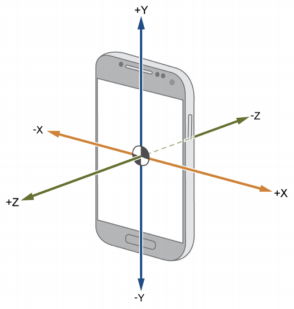
\includegraphics[width=\textwidth]{images/Mobile computing/1. Introduzione al Mobile Computing/accelerometro.PNG}
    \end{minipage} 
    \hfill
    \begin{minipage}{.5\textwidth}
        da una tripla di valori, uno per ciascun asse.
        Se tengo il device fermo e perfettamente in verticale, vedrò un asse che misura circa 1g (\begin{math} 9.8m/s^2 \end{math}) e gli altri circa 0g. Quando il dispositivo viene spostato, gli accelerometri misurano la combinazione della forza di gravità e dell'accelerazione dovuta effettivamente allo spostamento del dispositivo. Si può usare per conoscere la posizione del dispositivo rispetto a terra. Un esempio di utilizzo di accelerometro è la rotazione dello schermo
    \end{minipage}
    
    \item giroscopio: misura quanto rapidamente stiamo ruotando il device sui tre assi. Ogni lettura di valori, come per l'accelerometro, è una tripla di numeri e i valori di velocità vengono campionati nel tempo. Il giroscopio non misura l'accelerazione quindi non è influenzato dall'accelerazione di gravità. Se un dispositivo si trova in stato di quiete si avrà una lettura di valori prossimi allo zero su tutti e tre gli assi. Una cosa che non si riesce a fare con il giroscopio è darci una posizione
    \item magnetometro: è utile per capire dove sono orientato, rispetto al Nord magnetico terrestre. Misura i valori sui tre assi. Può avere una precisione molto bassa in particolari ambienti urbani. Non calcola la velocità di rotazione come il giroscopio, ma se usati in combinazione riusciamo a fornire un punto di orientamento assoluto (il giroscopio misura solo le rotazioni, ma non ha un orientamento di riferimento)
\end{itemize}

Ogni misurazione è soggetta ad errore. Il device non conosce l'errore ma possiamo misurarlo con strumenti esterni. 
\\ Una fonte d'errore nei sistemi inerziali è che vengono campionati i valori ad intervalli, ciò significa che i valori misurati dai sensori non sono acquisiti in modo costante. 

Anche la misurazione istantanea può essere soggetta ad errore. 

Spesso vogliamo usare i sensori inerziali per calcolare lo spostamento. 
\\ Usando i dati di accelerometri e giroscopi posso calcolare lo spostamento di un device con 6 gradi di libertà: 
\begin{itemize}
    \item 3 gradi di libertà per lo spostamento
    \item 3 gradi di libertà per l'orientamento
\end{itemize}
Il problema è che l'errore si accumula nel tempo e più tempo passa, più il calcolo dello spostamento è soggetto ad un errore maggiore. Questo effetto si chiama drift.

\subsubsection{Sensori di acquisizione immagini (fotocamere)}
Molti dispositivi mobili, in particolare smartphone e tablet, sono dotati di una o più videocamere per l’acquisizione di immagini e video.
Sono spesso utilizzate in molte applicazioni e servono per raccogliere informazioni dall'ambiente circostante e fornire altre funzionalità. Oltre che per scattare foto e registrare video possono essere usate in combinazione con le tecniche di visione artificiale. \\    Le applicazioni di queste tecniche sono numerose e includono: 
\begin{itemize}
    \item augmented-reality, per riconoscere il contesto attorno all'utente e mostrare elementi virtuali all'interno del mondo reale
    \item riconoscimento di oggetti
    \item sicurezza, ad esempio riconoscere il volto di una persona che sta cercando di sbloccare lo smartphone
    \item calcolo dello spostamento, usando una combinazione di sensori inerziali e dati della camera
\end{itemize}

Una caratteristica delle fotocamere è che sono in grado di calcolare le depth images. I pixel più chiari rappresentano oggetti più vicini. 
\\ Nella fotografia sono importanti quando ad esempio dobbiamo mettere a fuoco un soggetto, ma sono utili anche per comprendere l'ambiente.
\\ Nei dispositivi mobili le immagini di profondità possono essere calcolate con quattro approcci principali: 
\begin{itemize}
    \item stereo triangulation: come fa il cervello a calcolare la distanza dagli oggetti? Usando gli occhi, sfrutta le due immagini per vedere le differenze tra i due occhi e per calcolare la distanza.
    \\ La stessa cosa succede con le telecamere. Prendiamo due foto scattate dalle due fotocamere, le confrontiamo tra di loro e calcoliamo la distanza
    \item motion parallax: usiamo una sola camera per far finta di averne due. Prendo una foto in un certo istante, cerco di capire come si è spostato il device e dopo poco prendo un'altra immagine. 
    \\ Mi aspetto che quello che sto fotografando non si sia spostato di molto. 
    \item structured light: siamo in una stanza buia, dobbiamo calcolare la distanza tra una sorgente e un muro. Lanciamo due fasci di luce con un angolo noto da una sorgente. Faccio poi una foto al muro. Se il muro è molto vicino, i punti dei fasci sul muro saranno vicini. Se il muro è lontano, i due punti saranno lontani tra di loro.
    \item lidar: il funzionamento è simile a quello del radar. Il radar trasmette delle onde radio e in base a come ritornano posso calcolare quanto sono lontani gli oggetti. Nel lidar, invece, non vengono trasmesse onde radio, ma un laser
\end{itemize}

\subsubsection{Sensori virtuali}
Oltre ai sensori fisici i sistemi operativi dei dispositivi mobili rendono disponibili dei sensori virtuali, componenti software che simulano dei sensori fisici utilizzando i dati provenienti da altri sensori. 
\\ Un sensore virtuale è il contapassi, che non è un sensore vero e proprio, ma il SO acquisisce i dati dai sensori inerziali, li analizza, usa un algoritmo e rende disponibile al programmatore i passi contati. 

%%%%%%%%%%%%%%%%%%%%%%%%%%% QUARTA PARTE %%%%%%%%%%%%%%%%%%%%%%%%%%%
\section{Mobile computing}
I dispositivi mobili hanno introdotto una serie di problemi e opportunità che hanno richiesto uno sforzo tra tutte le discipline informatiche:
\begin{itemize}
    \item molti protocolli di \textbf{comunicazione di rete} sono stati studiati appositamente per i dispositivi mobili
    \item i \textbf{sistemi operativi} sono stati profondamente modificati per rispondere alle esigenze dei dispositivi mobili
    \item sono state introdotte nuove tecniche di \textbf{data management}, per trattare i dati dei dispositivi mobili, per esempio richiedendo lo sviluppo di \textbf{basi di dati} apposite che adottano nuovi \textbf{algoritmi e strutture dati} per trattare i dati spaziali e temporali generati dai dispositivi mobili
    \item nuove soluzioni sono state necessarie per adattare i \textbf{sistemi distribuiti} alle esigenze dei dispositivi mobili
    \item i dispositivi mobili hanno accentuato problemi relativi ai \textbf{linguaggi di programmazione} (es: la programmazione multi-piattaforma) ma al contempo hanno dato un impulso alla creazione di nuovi e moderni linguaggi
    \item i dispositivi mobili hanno richiesto di ri-progettare i paradigmi di \textbf{interazione uomo-macchina} e hanno evidenziato come gli aspetti di user-experience siano fondamentali per il successo commerciale delle applicazioni
    \item nuovi problemi e opportunità sono emersi nell’ambito della \textbf{sicurezza} (es., sistemi di riconoscimento biometrico applicati su larga scala), con un forte impatto anche su questioni di \textbf{privacy}
    \item i dispositivi mobili forniscono un nuovo contesto applicativo per gli ambiti della visione \textbf{artificiale}, del \textbf{machine learning}, della \textbf{grafica} e del \textbf{gaming}
\end{itemize}

\begin{comment}
Federichino

PDA = personal digital assistant




----------

Omarino





\end{comment}


